\documentclass[10pt]{article}
\usepackage[]{ragged2e}
\usepackage{fancyhdr,amsmath,amsthm,amssymb,bbm,graphicx,array,bm,tensor,braket,mathtools,tensor}
\usepackage{caption,subcaption,listings}
\usepackage{mathtools,tkz-euclide,slashed,url,hyperref}
\usepackage[utf8]{inputenc}
\usepackage[letterpaper,left=25mm,right=25mm,top=15mm]{geometry}

\setlength{\parskip}{1em}
\setlength{\parindent}{0em}

\newcommand{\Z}{\mathbb{Z}}
\newcommand{\R}{\mathbb{R}}
\newcommand{\Q}{\mathbb{Q}}
\newcommand{\C}{\mathbb{C}}
\newcommand{\N}{\mathbb{N}}

\DeclareMathOperator{\Ima}{Im}

\linespread{1.25}
%\pagestyle{fancy}
%\fancyhf{}
%\lhead{PHYS 921 $|$  Assignment 1}

%\rhead{Dilraj Ghuman $|$ 20191345}

% For code
\usepackage{xcolor}

\definecolor{codegreen}{rgb}{0,0.6,0}
\definecolor{codegray}{rgb}{0.5,0.5,0.5}
\definecolor{codepurple}{rgb}{0.58,0,0.82}
\definecolor{backcolour}{rgb}{0.95,0.95,0.92}

\lstdefinestyle{mystyle}{
    backgroundcolor=\color{backcolour},   
    commentstyle=\color{codegreen},
    keywordstyle=\color{magenta},
    numberstyle=\tiny\color{codegray},
    stringstyle=\color{codepurple},
    basicstyle=\ttfamily\footnotesize,
    breakatwhitespace=false,         
    breaklines=true,                 
    captionpos=b,                    
    keepspaces=true,                 
    numbers=left,                    
    numbersep=5pt,                  
    showspaces=false,                
    showstringspaces=false,
    showtabs=false,                  
    tabsize=2
}

\lstset{style=mystyle}


\begin{document}
\begin{center}
  {\Large \bf M\"{o}ssbauer Neutrino Oscillations}\\
  {\small \bf Dilraj Ghuman}
\end{center}
\vspace{2em}

\section{Introduction}

In 1958, M\"{o}ssbauer discovered recoil-less emission gammas in crystal structures. This behaviour allowed for certain resonance energies to be carried by the photons that would otherwise not be observed in the standard emission process. A natural progression would thus be to question whether this recoil-less process can be observed with other emission products, such as neutrinos. A potential process that could induce such an interaction would be the decay :
\[^{3} \textnormal{H} \to\,  ^{3}\textnormal{He} + e^{-} + \bar{\nu}_{e}\]
and the detection using the inverse process,
\[^{3}\textnormal{He} + e^{-} + \bar{\nu}_{e} \to\, ^{3} \textnormal{H}\, .\]
As these processes take place in a lattice, the text \cite{Akhmedov_2008} does cover some of these medium interactions. We only consider the dominant one as it is similar in the QFT formulation to the free space process. 

\section{External Wave-Packet Formalism}
In essence, the benefit of the \textit{external wave-packet formalism} is to treat the larger nuclei as external to the key internal interactions, like the anti-neutrino and electron in our case. For this reason, we can imagine a Feynman diagram that looks like figure \ref{fig:feyn}.

\tikzset{
  boson/.style={decorate, decoration={snake}},
  middlearrow/.style={
    decoration={markings,
      mark= at position 0.5 with {\arrow{#1}} ,
    },
    postaction={decorate}
  }
}

\begin{figure}[h]
  \centering
    \begin{tikzpicture}[scale=3]
    % Neutrino
    \draw [middlearrow={latex}] (0,0) -- (0.5,0);
    \node [above] at (0.25,0.1) {$\nu$};
    % H_D
    \draw [middlearrow={latex}] (0.5,0) -- (1,0.5);
    \node [right] at (1,0.5) {$\text{H}_{D}$};
    % He_D
    \draw [middlearrow={latex}] (1,-0.5) -- (0.5,0);
    \node [right] at (1,-0.5) {$\text{He}_{D}$};
    % H_S
    \draw [middlearrow={latex}] (-0.5,-0.5) -- (0,0);
    \node [left] at (-0.5,-0.5) {$\text{H}_{S}$};
    % He_S
    \draw [middlearrow={latex}] (0,0) -- (-0.5,0.5);
    \node [left] at (-0.5,0.5) {$\text{He}_{S}$};
    \end{tikzpicture}
    \caption{A simplified Feynman diagram of the interaction we are interested in.}
    \label{fig:feyn}
\end{figure}
In particular, if we follow along with Beuthe and Mikael \cite{Beuthe_2003}, they go through the Jacob-Sachs \cite{sachs} model. Though this model describes non-oscillating particles, \cite{Beuthe_2003} does eventually introduce oscillations as well. For this reason, we follow along with them. 

\subsection{Quantum Approach}
We have to first go through a simple formalism where we use quantum mechanics to get an estimate on the production rate of neutrinos without accounting for oscillations. We see in the paper that they reference the following hamiltonian for the tritium source decay
\begin{equation}\label{source_h}
  H_{S}^{+} = \int d^{3}x\frac{1}{\sqrt{2}}G_{F}\cos\theta_{c}\bra{^{3}\textnormal{He}}J^{\mu}\ket{^{3}\textnormal{H}}\bar{\psi}_{e,S}\gamma_{\mu}(1-\gamma^{5})\psi_{\nu},
\end{equation}
and the helium detection process,
\begin{equation}
  H_{D}^{-} = \int d^{3}x\frac{1}{\sqrt{2}}G_{F}\cos\theta_{c}\bra{^{3}\textnormal{H}}J^{\mu}\ket{^{3}\textnormal{He}}\bar{\psi}_{\nu}\gamma_{\mu}(1-\gamma^{5})\psi_{e,D}\, .
\end{equation}
To calculate the rate of neutrino production, we need to use these hamiltonians in combination with the ground state function(s):
\begin{equation}\label{ground_state}
  \psi_{A,B,0}(\bm{x}, t) = \left[\frac{m_{A},\omega_{A,B}}{\pi}\right]^{\frac{3}{4}}\exp\left[-\frac{1}{2}m_{A}\omega_{A,B}|\bm{x} - \bm{x}_{B}|^{2}\right]e^{-iE_{A,B}t}\, ,
\end{equation}
for $A \in \{\text{H}, \text{He}\}$ and $B\in \{S, D\}$ for the atom type and location respectively. Applying Fermi's golden rule,
\begin{align*}
  \Gamma_{i \to f} & = 2\pi|\bra{f}H_{I}\ket{i}|^{2}\rho(E_{f}) \\
  & = 2\pi|\bra{^{3}\text{He}_{S},\, ^{3}\text{H}_{D}}H_{S}^{+}\ket{^{3}\text{H}_{S},\, ^{3}\text{He}_{D}}|^{2}\rho(E_{f})
\end{align*}
where we need to replace the nuclear states with their corresponding ground state functions described in equation \ref{ground_state}. This is going to get ugly fast as everything is expanded, and this is before we evaluate the $\beta^{-}$ decay processes. In order to avoid becoming over encumbered in this first section (especially since it is before the QFT approach), we note that the leading coefficients to the $\Gamma_{0}$ term begin to appear as we factor out the $G_{F}$ and $\cos\theta_{c}$ terms. That being said, the final result takes the form
\begin{equation}
  \Gamma_{p} = \Gamma_{0}X_{S}\, ,
\end{equation}
where
\begin{equation}
  \Gamma_{0} = \frac{G^{2}_{F}\cos^{2}\theta_{c}}{\pi}|\psi(R)|^{2}m_{e}^{2}(|M_{V}|^{2}+g^{2}_{A}|M_{A}|^{2})\left(\frac{E_{S,0}}{m_{e}}\right)^{2}\kappa_{S}\, .
\end{equation}
To avoid repeating the paper reviewed, I won't explain the meaning of each term here other than the ones of interest to the derivation. The nuclear matrix elements $M_{V}$ and $M_{A}$ arise from the two different $\beta^{-}$ decay processes, Fermi and Gamow-Teller. The $X_{S}$ term carries the energy and mass terms (and hence the momentum) from the introduced groundstate wavefunctions for the source,
\begin{equation}
  X_{S} = 8\left(\eta_{S} + \frac{1}{\eta_{S}}\right)^{-3}e^{-\frac{p^{2}}{\sigma_{pS}^{2}}}
\end{equation}
where
\begin{equation}
  \eta_{S} = \sqrt{\frac{m_{\text{H}}\omega_{\text{H},S}}{m_{\text{He}}m_{\text{He},S}}}, \quad \sigma^{2}_{pS} = m_{\text{H}}\omega_{\text{H},S} + m_{\text{He}}\omega_{\text{He},S}\, .
\end{equation}
For the cross section, we consider the detection process and recall that the simplest relation of the differential cross-section is related to the scattering amplitude,
\begin{equation}
  \frac{d\sigma}{d\Omega}(\theta, \phi) = |f(\theta,\phi)|^{2}\, .
\end{equation}
We can follow along in \cite{bahcall, Akhmedov_2008} to get the final result as
\begin{equation}
  \sigma(E) = B_{0}X_{D}\delta(E - E_{D,0})\, ,
\end{equation}
where
\begin{equation}
  B_{0} = 4\pi G_{F}^{2}\cos^{2}\theta_{c}|\psi_{e}(R)|^{2}(|M_{V}|^{2} + g_{A}^{2}|M_{A}|^{2})\kappa_{D}\, .
\end{equation}
Here $X_{D}$ is the detection analogue of the source $X_{S}$. The text continues to then combine the production, propagation and detection processes to reach the total rate,
\begin{equation}
  \Gamma = \frac{1}{4\pi L^{2}}\int_{0}^{\infty}\rho(E)\sigma(E)dE \approx \frac{\Gamma_{0}B_{0}}{4\pi L^{2}}X_{S}X_{D}\frac{(\gamma_{S} + \gamma_{D})/2\pi}{(E_{S,0} - E_{D,0})^{2} + (\gamma_{S} + \gamma_{D})^{2}/4}\, ,
\end{equation}
where $\gamma_{S}$ and $\gamma_{D}$ are the energy widths assoiciated with production and detection. This result is used primarily as a comparison with the QFT treatment that is following.

\subsection{QFT Approach}
We want to use our standard Feynman rules for a weak interaction for the neutrino propagation using Figure \ref{fig:feyn}. We can start with the general form the amplitude (\cite{Beuthe_2003}) will take as being
\begin{align}
  \mathcal{A} & = \bra{f}\hat{T}\left(\exp\left(-i\int d^{4}x\mathcal{H}_{I}\right)\right) - \bm{1}\ket{i} \\
  & = \bra{^{3}\text{He}_{S},\, ^{3}\text{H}_{D}}\hat{T}\left(\exp\left(-i\int d^{4}x\mathcal{H}_{I}\right)\right) - \bm{1}\ket{^{3}\text{H}_{S},\, ^{3}\text{He}_{D}}\, ,
\end{align}
where $\mathcal{H}_{I}$ is the interaction lagrangian. Using equation \ref{ground_state} for the states in the bras and kets,
\begin{equation*}
  \mathcal{A} = \bra{^{3}\text{He}_{S},\, ^{3}\text{H}_{D}}\left(\int d^{3}x_{1}dt_{1}\ket{x_{1},t_{1}}\bra{x_{1},t_{1}}\right)\hat{T}\left(\exp\left(-i\int d^{4}x\mathcal{H}_{I}\right)\right)\left(\int d^{3}x_{2}dt_{2}\ket{x_{2},t_{2}}\bra{x_{2},t_{2}}\right)\ket{^{3}\text{H}_{S},\, ^{3}\text{He}_{D}}\, ,
\end{equation*}
but we associate $(x_{1},t_{1})$ with the source and $(x_{2},t_2)$ with the detector. It is also clear enough to see we can introduce another set of $(x_{1}',t_{1}')$ and $(x_{2}', t_{2}')$ to be completely rigorous in how our kets and bras pass by the propagator, but eventually have them removed using the inevitable $\delta$ functions that show up. As such, we get
\begin{align*}
  \mathcal{A} = \int & d^{3}x_{1}dt_{1}\int d^{3}x_{2}dt_{2}\braket{^{3}\text{He}_{S}|x_{1},t_{1}}\braket{x_{1},t_{1}|\,^{3}\text{H}_{S}}\braket{^{3}\text{H}_{D}|x_{2},t_{2}}\braket{x_{2},t_{2}|\,^{3}\text{He}_{D}} \\
  & \cdot \bra{x_{1}, t_{1}}\hat{T}\left(\exp\left(-i\int d^{4}x\mathcal{H}_{I}\right)\right)\ket{x_{2},t_{2}} \, ,
\end{align*}
and subbing in the states,
\begin{align*}
  \mathcal{A} = \int & d^{3}x_{1}dt_{1}\int d^{3}x_{2}dt_{2} \left(\frac{m_{\text{He}},\omega_{\text{He},S}}{\pi}\right)^{\frac{3}{4}}\exp\left[-\frac{1}{2}m_{\text{He}}\omega_{\text{He},S}|\bm{x}_{1} - \bm{x}_{S}|^{2}\right]e^{iE_{\text{He},S}t_{1}}\\
  & \cdot \left(\frac{m_{\text{H}},\omega_{\text{H},S}}{\pi}\right)^{\frac{3}{4}}\exp\left[-\frac{1}{2}m_{\text{H}}\omega_{\text{H},S}|\bm{x}_{1} - \bm{x}_{S}|^{2}\right]e^{-iE_{\text{H},S}t_{1}} \\
  & \cdot \left(\frac{m_{\text{H}},\omega_{\text{H},D}}{\pi}\right)^{\frac{3}{4}}\exp\left[-\frac{1}{2}m_{\text{H}}\omega_{\text{H},D}|\bm{x}_{2} - \bm{x}_{D}|^{2}\right]e^{iE_{\text{H},D}t_{2}}\\
  & \cdot \left(\frac{m_{\text{He}},\omega_{\text{He},D}}{\pi}\right)^{\frac{3}{4}}\exp\left[-\frac{1}{2}m_{\text{He}}\omega_{\text{He},D}|\bm{x}_{2} - \bm{x}_{D}|^{2}\right]e^{-iE_{\text{He},D}t_{2}}\\
  & \cdot \bra{x_{1}, t_{1}}\hat{T}\left(\exp\left(-i\int d^{4}x\mathcal{H}_{I}\right)\right)\ket{x_{2},t_{2}} \, .
\end{align*}

This is beginning to look like the transition amplitude in the text \cite{Akhmedov_2008}. The difficult part begins now in attempting to understand the propagator in this weak interaction with external atoms. It is simplest here to use the Feynman rules for the relevant vertices. We note there will be contributions from the tritium decay, the inverse process, and the propagation of the neutrino and electron. Though all the processes aside from the neutrino are external, they still will complicate this. First, we note that our neutrino is a fermion, so we know the propagator is of the form,
\begin{equation}
  \Pi = \frac{i(\slashed{p} + m_j)}{p_{0}^{2}-\bm{p}^{2} - m_{j}^{2} + i\epsilon}\, ,
\end{equation}
where the $j$ index will relate to the PMNS matrix for oscillations. Next, we need to account for the charged current vertices where our lepton and neutrino interact. Luckily, this is a well known vertex in texts \cite{ew_lec} and takes the form
\begin{equation}
  \mathcal{V} = -i\frac{g}{2\sqrt{2}}\gamma_{\mu}(1 - \gamma_{5}) \, .
\end{equation}
Moreover, we need to account for the external electron as a Dirac spinor using $u_{e,D}$ and $u_{e,S}$ where the first index is for the electron and the second is for the location. We can similarly account for the Helium and Tritium with $u_{\text{He}}$ and $u_{\text{H}}$ respectively. Putting these together, we get
\begin{equation}
  \mathcal{B} = -\left(\frac{g}{2\sqrt{2}}\right)^{2}\int \frac{d^{4}p}{(2\pi)^{4}}e^{-ip_{0}(t_{2} - t_{1}) + i\bm{p}(\bm{x}_{2} - \bm{x}_{1})}\bar{u}_{e,S}\gamma_{\mu}(1-\gamma_{5})\frac{i(\slashed{p} + m_j)}{p_{0}^{2}-\bm{p}^{2} - m_{j}^{2} + i\epsilon}(1 + \gamma_{5})\gamma_{\nu}u_{e,D} \, .
\end{equation}
Now we have to account for the tritium and helium terms in their decay and capture interactions respectively. The vertex of interest is provided by Figure \ref{fig:decay}.

\begin{figure}[h]
  \centering
  \begin{tikzpicture}[scale=3]
    % Neutrino
    \draw [boson] (0,0) -- (0.5,0);
    \node [above] at (0.25,0.1) {$W^{-}$};
    % lepton
    \draw [middlearrow={latex}] (0.5,0) -- (1,0.5);
    \node [right] at (1,0.5) {$e^{-}$};
    % neutrino
    \draw [middlearrow={latex}] (1,-0.5) -- (0.5,0);
    \node [right] at (1,-0.5) {$\bar{\nu}_{e}$};
    % H
    \draw [middlearrow={latex}] (-0.5,-0.5) -- (0,0);
    \node [left] at (-0.5,-0.5) {$\text{H}$};
    % He
    \draw [middlearrow={latex}] (0,0) -- (-0.5,0.5);
    \node [left] at (-0.5,0.5) {$\text{He}$};
  \end{tikzpicture}
  \caption{The decay of Tritium}
  \label{fig:decay}
\end{figure}

The acting interaction in this is the neutron decay into a proton, where one of the down quarks changes to an up quark via a neutral or charged current interaction. This $\beta^{-}$ decay is incredibly important and is how Fermi postulated the existence of neutrinos to begin with \cite{ft_beta}. So, in order to understand how this Matrix element may look, we look at the pieces involved.

First, we note that we should expect a V-A type theory, as it is the general form when considering a spin-1 particle exchange \cite{ft_beta}. For this reason, we can expect that the matrix element for the Tritium decay to be of the form
\begin{equation}
  \mathcal{M}_{D}^{\mu} \sim M_{V} - g_{A}M_{A}
\end{equation}
where there are some missing factors. Here we have denoted $M_{V}$ and $M_{A}$ as the nuclear vector and axial-vector matrix elements with $g_{A}$ as the axial-vector coupling constant. This is similar to what was discussed in the Quantum section. To get closer to the result in the text, we note that we want to associate the vector and axial component with certain parts of the propagation. For this neutrino source, we want to contract these with $\gamma_{\mu}$, and so more explicitly
\begin{equation}
  \mathcal{M}_{D}^{\mu} \sim M_{V}\delta^{\mu}_{0} - g_{A}M_{A}\sigma_{i}\delta^{\mu}_{i}/\sqrt{3}\, .
\end{equation}
The $\delta^{\mu}_{0}$ pulls the vector like components of our $\gamma_{\mu}$ and the $\sigma_{i}\delta^{\mu}_{i}$ pulls the axial-vector (the twisting) part, where $\sigma_{i}$ are the traditional pauli-matrices.   

Next we want to treat the external Helium and Tritium as external spin-$\frac{1}{2}$ particles, so
\begin{equation}
  \mathcal{M}_{D}^{\mu} \sim \bar{u}_{\text{He}}\left(M_{V}\delta^{\mu}_{0} - g_{A}M_{A}\sigma_{i}\delta^{\mu}_{i}/\sqrt{3}\right)u_{\text{H}}\, .
\end{equation}
Looking at equation \ref{source_h}, we see that we better get a leading factor that looks like $\frac{G_{F}\cos\theta_{c}}{\sqrt{2}}$. Comparing with the text \cite{Akhmedov_2008} we note we have the $\psi_{e}(R)$ and $\kappa_{D}^{1/2}$ left, which are the wavefunctions of the external electron and Tritium/Helium products. Looking at \cite{Beuthe_2003}, we see these terms arise out of the overlap between the incoming and outgoing states.

Finally, before we can tie it all together, we need to account for the mass mixing of the propagating neutrino. Referring to \cite{Beuthe_2003}, in order to utilize the propagator as we have in the mass basis, we need to transform from the flavour basis propagator to the mass basis free propagator:
\begin{equation}
  G_{\beta\alpha}(x' - x) = \sum_{j}U_{\beta j}^{\dagger}G_{jj}(x' - x)U_{j\alpha}\,,
\end{equation}
where $G_{\beta\alpha}(x' - x)$ is the flavour basis propagator and $G_{jj}(x' - x)$ is the free propagator of a particle with mass $m_{j}$. Note that we must have the PMNS mixing matrix take us between these bases, $U_{ij}$. In our case, we know that the lepton produced is an electron, so this will immediately fix one of our indices. However, we must now sum over the remain index to account for the mixing of the neutrino. This is described in \cite{Beuthe_2003} as being the result of being unable to treat the oscillations as local property, and instead requiring them to be a global property (as otherwise we fail to observe them at all).

So, we get the final result matching the text \cite{Akhmedov_2008},
\begin{equation}\label{eq:final}
  \begin{split}
  i\mathcal{A} = \int & d^{3}x_{1}dt_{1}\int d^{3}x_{2}dt_{2} \left(\frac{m_{\text{He}},\omega_{\text{He},S}}{\pi}\right)^{\frac{3}{4}}\exp\left[-\frac{1}{2}m_{\text{He}}\omega_{\text{He},S}|\bm{x}_{1} - \bm{x}_{S}|^{2}\right]e^{iE_{\text{He},S}t_{1}}\\
  & \cdot \left(\frac{m_{\text{H}},\omega_{\text{H},S}}{\pi}\right)^{\frac{3}{4}}\exp\left[-\frac{1}{2}m_{\text{H}}\omega_{\text{H},S}|\bm{x}_{1} - \bm{x}_{S}|^{2}\right]e^{-iE_{\text{H},S}t_{1}} \\
  & \cdot \left(\frac{m_{\text{H}},\omega_{\text{H},D}}{\pi}\right)^{\frac{3}{4}}\exp\left[-\frac{1}{2}m_{\text{H}}\omega_{\text{H},D}|\bm{x}_{2} - \bm{x}_{D}|^{2}\right]e^{iE_{\text{H},D}t_{2}}\\
  & \cdot \left(\frac{m_{\text{He}},\omega_{\text{He},D}}{\pi}\right)^{\frac{3}{4}}\exp\left[-\frac{1}{2}m_{\text{He}}\omega_{\text{He},D}|\bm{x}_{2} - \bm{x}_{D}|^{2}\right]e^{-iE_{\text{He},D}t_{2}}\\
  & \cdot\sum_{j}\mathcal{M}^{\mu}_{S}\mathcal{M}^{\nu *}_{D}|U_{ej}|^{2}\mathcal{B} \, .
  \end{split}
\end{equation}

To simplify, we note that the time integrals should be relatively simple using 
\begin{equation}
  \frac{1}{2\pi}\int dt e^{itE} = \delta(E) \, ,
\end{equation}
as this tells us that the integrals over the $t_{1}$ and $t_{2}$ variables will pull out delta functions for energy conservation at the source and detector (note these integrals will also include the exponential with $t_{1}$ and $t_{2}$ in $\mathcal{B}$). The spatial integrals are Gaussian under the transformation of $\bm{x}_{1} \to \bm{x}_{1} + \bm{x}_{S}$ and $\bm{x}_{2} \to \bm{x}_{2} + \bm{x}_{D}$, and using the identity
\begin{equation}
  \int_{-\infty}^{\infty} dx e^{-ax^{2}} = \sqrt{\frac{\pi}{a}}\,
\end{equation}
we are left with a leading factor of
\begin{align*}
  \mathcal{C} = & (2\pi)^{2}\delta(p_{0} - (E_{\text{He},S} - E_{\text{H},S}))\delta(p_0 - (E_{\text{H},D} - E_{\text{He},D}))\sqrt{\frac{2\pi}{(m_{\text{H}}\omega_{\text{H},S} + m_{\text{He}}\omega_{\text{He},S})}}\sqrt{\frac{2\pi}{(m_{\text{H}}\omega_{\text{H},D} + m_{\text{He}}\omega_{\text{He},D})}}\, .  
\end{align*}
Comparing with \cite{Akhmedov_2008}, we see there is a slight discrepancy in the factor they define as $\mathcal{N}$, as that is where they push all the cumbersome coefficients. They seem to disagree on the degree of the
\[ \sqrt{\frac{2\pi}{(m_{\text{H}}\omega_{\text{H},S} + m_{\text{He}}\omega_{\text{He},S})}}\sqrt{\frac{2\pi}{(m_{\text{H}}\omega_{\text{H},D} + m_{\text{He}}\omega_{\text{He},D})}} \]
terms; where my terms have exponents of $\frac{1}{2}$, the text has $\frac{3}{2}$. These Gaussian integrals should be relatively straightforward, unless I made an obvious error. Regardless, the difference is noted.

From here, the text \cite{Akhmedov_2008} uses a theorem by Grimus and Stockinger \cite{Grim} which in the limit we push the detection and source positions far enough away, we get an approximation to leading order in $1/L$, with $L$ the length between the two points. This gives
\begin{align*}
  i\mathcal{A} = & \frac{-i}{2L}\mathcal{N}\delta(E_{S} - E_{D})\sum_{j}\exp\left[-\frac{E_{S}^{2} - m_{j}^{2}}{2\sigma^{2}_{p}}\right]\mathcal{M}_{S}^{\mu}\mathcal{M}_{D}^{\nu *}|U_{ej}|^{2}e^{i\sqrt{E_{S}^{2} - m_{j}^{2}}L} \\
  & \cdot \bar{u}_{e,S}\gamma_{\mu}(1-\gamma^{5})(\slashed{p}_{j} + m_{j})(1 + \gamma^{5})\gamma_{\nu}u_{e,D}\, .
\end{align*}

\section{M\"{o}ssbauer Neutrinos and the Natural Linewidth}

We now skip to the section where the text \cite{Akhmedov_2008} speaks of the dominating effect in the crystal structure. In particular, the decays of the unstable nuclei are introduced into the amplitude found in equation \ref{eq:final} as exponential decay factors of the form
\begin{equation}
  e^{-\gamma t/2} \hspace{2em} \& \hspace{2em} e^{-\gamma(T-t_{2})/2}
\end{equation}
for tritium in the source and detector respectively. Here, $t$ is the time after the experiment has started, $t_{2}$ the production time, $T$ is the time at which the number of produced tritium atoms is counted and $\gamma$ is the total decay width of tritium. Following a procedure similar to the above, the text finds the total probability of finding a tritium atom at the at the position $\bm{x}_{D}$ after a time $T$ as
\begin{equation}\label{eq:prob_before}
  \begin{split}
    \mathcal{P} = \frac{\Gamma_{0}B_{0}}{4\pi L^{2}} & Y_{S}Y_{D}\frac{2}{\pi}\sum_{j,k}\theta(T_{jk})|U_{ej}|^{2}|U_{ek}|^{2} \\
    & \cdot \exp\left[-\frac{(p_{jk}^{\text{min}})^{2}}{\sigma_{p}^{2}}\right]\exp\left[-\frac{|\Delta m_{jk}^{2}|}{2\sigma^{2}_{p}}\right]e^{i\left(\sqrt{\bar{E}^{2} - m_{j}^{2}} - \sqrt{\bar{E}^{2} - m_{k}^{2}}\right)L} \\
    & \cdot e^{-\gamma T_{jk}}e^{-L/L_{jk}^{\text{coh}}}\frac{\sin\left[\frac{1}{2}(E_{S,0} - E_{D,0})(T - \frac{L}{v_{j}})\right]\sin\left[\frac{1}{2}(E_{S,0} - E_{D,0})(T - \frac{L}{v_{k}})\right]}{(E_{S,0} - E_{D,0})^{2}}\, .
  \end{split}
\end{equation}
Now that we have this, since I am not a theorist and don't expect myself to be able to do any ground-breaking work for this project, I resort to trying to plot a grossly approximated total probability in arbitrary units. To do this, I'll describe what the terms mean, and which ones I'll be ignoring for the sake of simplicity.

First off, to avoid repeating and as a comparison, we consider the approximation given in the text itself. In the case of SM neutrinos (so zero mass and hence no oscillations), we see that the probability reduces to being proportional to
\begin{equation}
  e^{-\gamma T}\frac{\sin^{2}[(E_{S,0} - E_{D,0})\frac{T}{2}]}{(E_{S,0} - E_{D,0})^{2}}\, .
\end{equation}

To compare with this, we take another approximation pathway. First, we ignore all the leading factors as they are constant and don't change the shape of the plots. Next we need to consider the oscillation matrix elements. Ignoring these would effectively reduce to the SM case, so we have to keep some form of oscillations. Instead, we make the approximation that $|\Delta m_{jk}^{2}| \ll 1$, so this changes $p_{jk}^{\text{min}} = \bar{E}^{2} - \text{max}(m_{j}^{2},m_{k}^{2}) \approx \bar{E}^{2} - m^{2} = \text{const}$, and hence we can ignore that corresponding exponential term as well. Continuing on this train of thought, we see this approximation naturally drops the exponential that involves $\left(\sqrt{\bar{E}^{2} - m_{j}^{2}} - \sqrt{\bar{E}^{2} - m_{k}^{2}}\right)$ to the identity. The other exponential we leave as it is. We note this will depend upon the spread $\sigma_{p}$, which is defined in the text as a combination of the $m_{A}$ and $\omega_{A,B}$ type terms. Regardless it is constant and we can fix it for the sake of plotting.

Next, we note that
\begin{equation}
  T_{jk} = \text{min}\left(T - \frac{L}{v_{j}}, T - \frac{L}{v_{k}}\right)
\end{equation}
compares the arrival time of the first neutrino to the total runtime. The heaviside function $\theta(T_{jk})$ ensures that both mass eigenstates arrive within the run time $T$. The final factor of importance is
\begin{equation}
  \frac{1}{L_{jk}^{\text{coh}}} = \gamma\left |\frac{1}{v_{j}} - \frac{1}{v_{k}}\right|\, ,
\end{equation}
which is just a coherence factor of the group velocities of the neutrinos. For the ultra-relativistic case (which is similar to the approximation we are taking), the text \cite{Akhmedov_2008} tells us that it should approximate to
\begin{equation}
  L_{jk}^{\text{coh}} = \frac{4\bar{E}^{2}}{\gamma|\Delta m_{jk}^{2}|}\,.
\end{equation}

It is important we look at the group velocities as well. Here we have defined them as
\begin{equation}
  v_{j} = \frac{\left(\bar{E}^{2} - m_{j}^{2}\right)^{\frac{1}{2}}}{\bar{E}}\, .
\end{equation}
We look at the ratio of two of these velocities,
\begin{equation}
  \begin{split}
    \frac{v_{j}}{v_{k}} & = \frac{\left(\bar{E}^{2} - m_{j}^{2}\right)^{\frac{1}{2}}}{\left(\bar{E}^{2} - m_{k}^{2}\right)^{\frac{1}{2}}} \\
    & = \left(\bar{E}^{2} - m_{j}^{2}\right)^{\frac{1}{2}}\left(\bar{E}^{2} - m_{k}^{2}\right)^{-\frac{1}{2}} \\
    & = \left(1 - \frac{m_{j}^{2}}{2\bar{E}^{2}} + \mathcal{O}(m_{j}^{4})\right)\left(1 + \frac{m_{k}^{2}}{2\bar{E}^{2}} + \mathcal{O}(m_{k}^{4})\right) \\
    & \approx 1 - \frac{\Delta m_{jk}^{2}}{2\bar{E}} \, .
  \end{split}
\end{equation}
Now if we use our approximation $|\Delta m_{jk}^{2}| \ll 1$, this will reduce to $1$, and will effectively take us back to the SM approximation. So, in this case, we choose not to take this approximation, and instead for plotting purposes we decide $\bar{E} = \frac{1}{2}$, and since $\bar{E} = \frac{1}{2}(E_{S,0} + E_{D,0})$, we can plot the difference $(E_{S,0} - E_{D,0})\in \{-1, 1\}$. Unfortunately this isn't exactly enough to compute $T_{jk}$, as we still need some method of computing the group velocities that aren't just ratios. So, we will have to fix one of the velocities. The only reasonable choice is to fix the lightest mass and computing the other three from there, so we let $v_{1} = 1$. Then
\begin{equation}
  v_{2} = \left(1 - \Delta m_{21}^{2}\right)v_{1} \hspace{2em} \& \hspace{2em} v_{3} = \left(1 - \Delta m_{32}^{2}\right)v_{2}\,.
\end{equation}

Now, the only thing left to do before plotting is to figure out the matrix elements $|U_{ej}|^{2}$. From the PDG \cite{pdg_true}, we can get the relations of these elements to the oscillation parameters, and rearranging we get
\begin{equation}
  |U_{e3}|^{2} = \sin^{2}\theta_{13}\, , \quad |U_{e2}|^{2} = (1-\sin^{2}\theta_{13})\sin^{2}\theta_{12}\, , \quad |U_{e1}|^{2} = (1-\sin^{2}\theta_{13})(1 - \sin^{2}\theta_{12})
\end{equation}
where we can get the values for the sinusoidals using the PDG \cite{pdg_true} as well (to some best fit of recent experiments). We choose the normal ordering.

So, for completeness, we will be plotting the following,
\begin{equation}
  \begin{split}
    \mathcal{P} \propto & \sum_{j,k}\theta(T_{jk})|U_{ej}|^{2}|U_{ek}|^{2}\exp\left[-\frac{|\Delta m_{jk}^{2}|}{2\sigma^{2}_{p}}\right]e^{-\gamma T_{jk}}e^{-L/L_{jk}^{\text{coh}}} \\
    & \cdot \frac{\sin\left[\frac{1}{2}(E_{S,0} - E_{D,0})(T - \frac{L}{v_{j}})\right]\sin\left[\frac{1}{2}(E_{S,0} - E_{D,0})(T - \frac{L}{v_{k}})\right]}{(E_{S,0} - E_{D,0})^{2}}\, .
  \end{split}
\end{equation}

\begin{figure}
  \centering
  \begin{subfigure}[b]{0.4\textwidth}
    \centering
    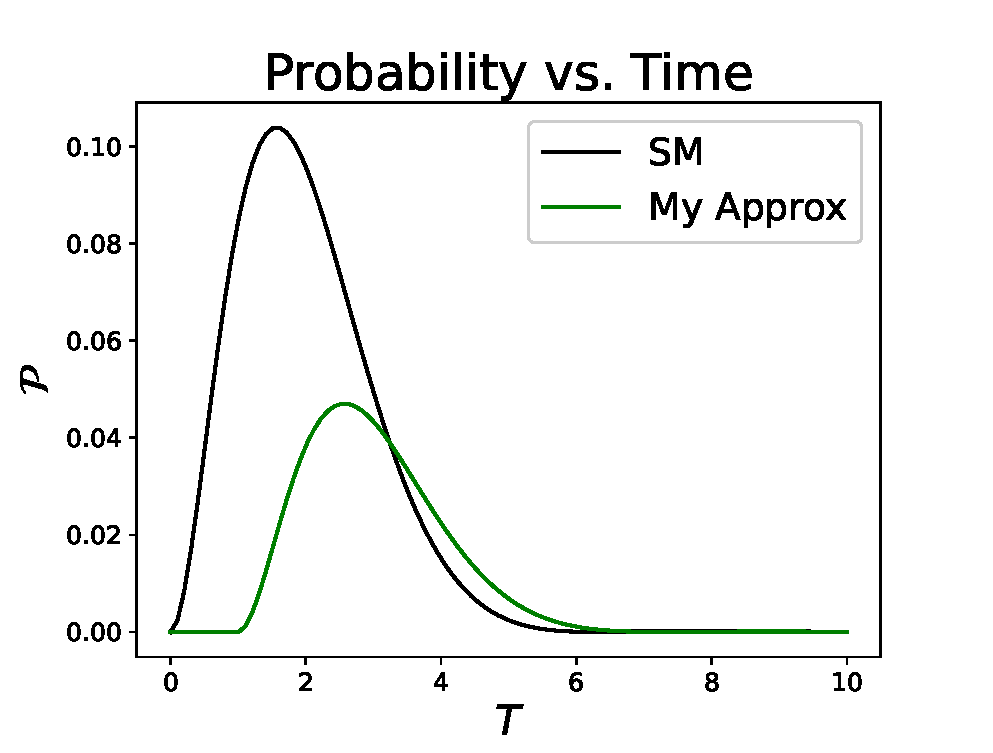
\includegraphics[width=\textwidth]{plots/T_plot.eps}
    \caption{Plotting time (in arbitrary units) against Probability.}
    \label{fig:time}
  \end{subfigure}
  \hspace{2em}
  \begin{subfigure}[b]{0.4\textwidth}
    \centering
    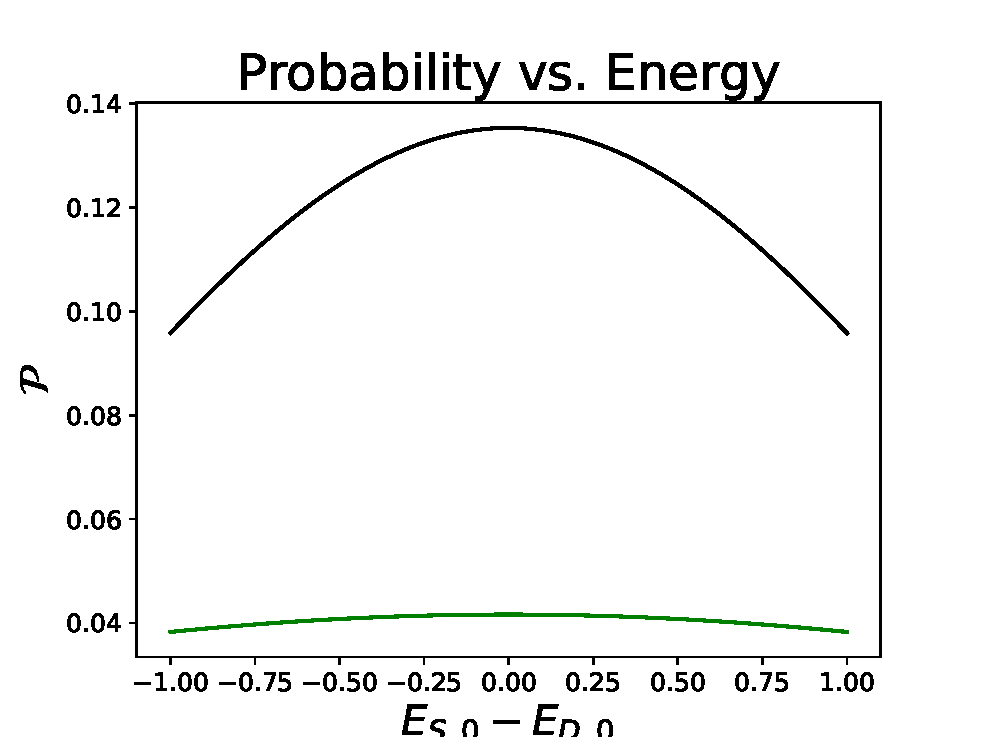
\includegraphics[width=\textwidth]{plots/E_plot.eps}
    \caption{Plotting the energy difference $E_{S,0} - E_{D,0}$ against Probability.}
    \label{fig:energy}
  \end{subfigure}
  \caption{Two simple plots to get an idea of the difference between the two approximations.}
  \label{fig:plots}
\end{figure}

Looking at Figure \ref{fig:plots} we see the results of comparing the two approximation methods. In particular, the largest difference seems to occur in the timing. The probability of finding a tritium atom at the site $\bm{x}_{D}$ peaks later in my approximation method compared to the SM approximation used in the text. From looking at the equations, we can guess this is due to the requirement that for a contribution to be included, we need both mass states to have arrived by the time $T$.

As a note, I didn't mess with the other parameters in the code. However they have been set such that more indepth plotting could be done to see the behaviour of this probability as we vary those other parameters.

\section{Conclusion}

The derivation of oscillations in M\"{o}ssbauer neutrinos is a deep-dive into understanding the interactions between nuclei and their decay particles.  In order to make this approachable, we used an external wave-packet methodology to be able to account for the external capture and decay nuclei. We then took those interaction Hamiltonians and built a QFT.

Looking at the dominating process, we took the probability of observing a Tritium nucleus at the detection sight, $\bm{x}_{D}$, and looked into a way of plotting it. I made another approximation including the oscillation parameters (to the best of my ability) to compare with the SM neutrinos approximation. We observed that the largest discrepancy lay primarily in the timing, where the probability of observing this tritium atom peaked later when we included some oscillations. The energy distributions showed that we expected a peak when $E_{S,0} = E_{D,0}$ as expected, since this tells us the largest probability will be when the energies are at resonance. 

Though it should have been obvious, I was still surprised by how much I still have to learn about QFT. The course was able to provide an introductory base to understanding how we can go about taking an interaction theory and building a full QFT, but the subtleties of applying that to a much more complex theory was a big leap. Regardless, I enjoyed working on the project and getting a better appreciation of QFTs in the `real world'.

\newpage
\section{Appendix}
I include the code I wrote to make the plots in Figure \ref{fig:plots}:

\lstinputlisting[language=Python]{code/plot.py}

%\end{lstlisting}


\newpage
%\bibliographystyle{prsty}
\bibliographystyle{plain}

\bibliography{bib}


\end{document}
